
\documentclass[12pt]{article}
\usepackage{graphicx}

\title{PROGRAMMING LANGUAGES}
\author{Timothy Eyo}

\begin{document}
	\maketitle
	\newpage
	\section*{\Huge{JAVA}}
		\begin{figure}
			\centering
			\includegraphics[width=0.7\linewidth]{"kisspng-logo-java-development-kit-portable-network-graphic-5d0f25d6adc385.3528057515612738147117 (2)"}
			\caption{JAVA}
			\label{fig:kisspng-logo-java-development-kit-portable-network-graphic-5d0f25d6adc385}
\end{figure}
	    \begin{minipage}{0.59\linewidth}
	    	\paragraph{Founder}
	        James Arthur Gosling, also referred to “Dr. Java”, is a Canadian computer scientist renown as the lead developer of the Java programming language. He was born on the 19th of May, 1955. He attended William Aberhart High School and received a Bachelor of Science from the University of Calgary and his M.A and Ph.D. from Carnegie Mellon University, all in computer science. He created the original design for Java and implemented the language’s original compiler and virtual machine.
	    	
	    	\textbf{\large}
	    \end{minipage}
       
    \subsection*{\Large \underline{History of Java}}
           \paragraph{}
           Java team members (also known as the Green team) initially developed the language for digital devices such as televisions and set-up boxes. However its developers soon discovered that it was best suited for programming. James Gosling, known as the father of Java, developed the language in 1995. Java technology was incorporated by Netscape. Today, Java is used in internet programming, mobile devices, games, e-businesses, etc.   
    \subsection*{\underline{Applications}}
            \paragraph{}
            Java has a wide range of uses. Some of these include:
            \begin{enumerate}
            	\item Mobile app development.
            	\item Game development.
            	\item Cloud-based apps.
            	\item IoT applications.
             \end{enumerate}
             \paragraph{}
             Future applications include:
             \begin{enumerate}
             	\item Block-chain technology.
             	\item Artificial Intelligence.
             \end{enumerate}       
    \subsection*{\underline{Available IDEs}}
            \paragraph{}
            These include:
            \begin{enumerate}
            	\item Eclispe.
            	\item BlueJ.
            	\item jGRASP.
            	\item JCreator.
            	\item NetBeans.
            	\item Greenfoot.
            	\item JDeveloper, etc.
            \end{enumerate}
     \subsection*{\underline{Related Programming Languages}}
            \paragraph{}
            Some programming languages similar to Java are:
            \begin{enumerate}
            	\item Kotlin.
            	\item Scala.
            	\item Python.
            	\item Go.
            \end{enumerate}
    \newpage
    \section* {\Huge{CSS}}
		\begin{figure}
		\centering
		
\includegraphics[width=0.7\linewidth]{CSS.logo}
		\caption{}
		\label{fig:css}
		\end{figure}
           \begin{minipage}{\linewidth{0.39}
                \paragraph{Founder}
                Hakon Wium Lie is a Norwegian web pioneer, a standard activist, and the chief technology officer of Opera Software from 1998 until the browser was sold to new owners in 2016. He was born on the 16th of July, 1965. He attended Ostfold University College, West Georgia College, and MIT Media Lab. He received an MS in visual studies in 1991. While working with Tim Bernards-Lee and Robert Cailliau at CERN in 1994, he proposed the concept of the Cascading Style Sheets (CSS).
                \textbf{\large}
            \end{minipage}
            \begin{minipage}{\linewidth{0.39}}
           	\end{minipage}           
            \subsection*{\Large \underline{History of CSS}}
                   \paragraph{}
                       CSS (Cascading Style Sheets) was first proposed by Hakon Wium Lie on the 10th of October, 1994. At the time he was working with Tim-Berners Lee at CERN. He presented his proposal at the Mosaic and the Web Conference at Chicago as a style sheet language for the web in 1994 and again with Bert Bos in 1995. The W3C took an interest in the development of CSS and organized a workshop. Lie and Bos were the lead technical staff with additional members participating as well. By the end of 1996, CSS was ready to become official.                                     
            \subsection*{\underline{Applications}}
                   \paragraph{}
                   CSS is mainly used web development. It popularly used to define the styles of web pages. This includes:                   
                   \begin{enumerate}
                   	   \item Web Development.
                   	   \item Website layout design.
                   	   \item Text color.
                   	   \item Paragraph spacing.
                   \end{enumerate}               
               \subsection*{\underline{Available IDEs}}
                      \paragraph{}
                      Popular IDEs for CSS include:                      
                      \begin{enumerate}
                      	\item Sublime Text.
                      	\item Text Pad.
                      	\item BBEdit.
                      	\item Komodo IDE.
                      	\item Visual Studio Code.
                      	\item Atom, etc.
                      \end{enumerate}               
               \subsection*{\underline{Related Programming Languages}
               	      \paragraph{}
               	      Some similar programming languages are:     	      
               	      \begin{enumerate}
               	      	\item Sass.
               	      	\item Bootstrap.
               	      	\item JavaScript.
               	        \item Python.
               	        \item PHP.
               	      \end{enumerate}                  
    \newpage
    \section* {\Huge{HTML}}
		\begin{figure}
		\centering
		
\includegraphics[width=0.7\linewidth]{html.logo}
		\caption{}
		\label{fig:html}
		\end{figure}
            \begin{minipage}{\linewidth{0.59}}
                       	   \paragraph{Founder}
                       	       \textbf{\large Timothy John Bernards-Lee was born on the 8th of June, 1955 in London, England. He attended Sheen Mount Primary School and then later went on to attend south-west London’s Emanuel School. He studied at The Queen’s College, Oxford from 1973 to 1976, where he received a first class Bachelor of Arts degree in Physics.}
            \end{minipage}
            \begin{minipage}{\linewidth{0.39}}
	\begin{figure}
		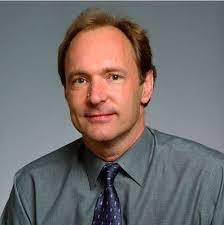
\includegraphics[width= \linewidth]{tim-berners-lee.jpg}
	`	\caption{}
		\label{fig:tim-berners-lee}
	\end{figure}
                           \end{minipage}
                       \subsection*{\Large \underline{History of HTML}}
                              \paragraph{}
                                  HTML (Hyper Text Mark-up Language) was invented by Tim Bernards-Lee, a physicist at CERN research institute in 1991. It is a mark-up language that web browsers use to interpret and compose text, images and other material into visual and audible web pages. He first proposed and prototyped ENQUIRE, a system for CERN researchers to use and share documents in 1980. The first publicly available description of HTML was a document called “HTML Tags”, first mentioned by Tim Benards-Lee in late 1991. It described 18 elements comprising the initial, relatively simple design of HTML.                              
                         \subsection*{\underline {Applications of HTML}}
                              \paragraph{}
                               HTML is popularly used to construct web pages. It is used along side CSS to:
                              \begin{enumerate}
                              	\item Design text.
                              	\item Organize illustrations.
                              	\item Connect to various pages inside a site.
                              \end{enumerate}                          
                       \subsection*{\underline {Available Integrated Development Environments (IDEs)}}
                              \paragraph{}
                              HTML IDEs include:                              
                              \begin{enumerate}
                              	\item Sublime Text 3.
                              	\item Komodo IDE.
                              	\item Codeanywhere.
                              	\item WebStorm.
                              	\item PhpStorm.
                              	\item Visual Studio, etc.
                              \end{enumerate}                          
                       \subsection*{\underline {Related Programming Languages}
                       	      \paragraph{}
                       	      Alternative programming languages include:    	      
                       	      \begin{enumerate}
                       	      	\item C/C++.
                       	      	\item PHP.
                       	      	\item Ruby.
                       	      	\item Pyhton.
                       	      	\item CSS.
                       	      \end{enumerate}                      
    \newpage
    \section* {\Huge{C#}}
		\begin{figure}
			\centering
			
\includegraphics[width=0.7\linewidth]{c#.logo}
			\caption{}
			\label{fig:c}
		\end{figure}
                               \begin{minipage}{\linewidth{0.59}}
                               	   \paragraph{Founder}
                               	    Anders Hejlsberg is a Danish software engineer, who currently works in Microsoft as the lead architect of C# and core developer of TypeScript. 
                               	   \textbf{\Large}
                               \end{minipage}
                           \begin{minipage}{linewidth{0.39}}
		\begin{figure}
			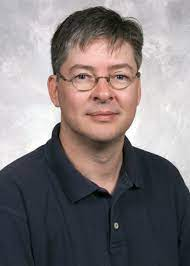
\includegraphics[width \linewidth]{anders}
			\caption{}
			\label{fig:anders}
		\end{figure}
                           \end{minipage}
                         \subsection* {\underline{History of C\#}}
                              \paragraph{}
                                  C\# was developed by Anders Hejlsberg and his team from Microsoft in 2000. The language was part of the NET project to build a new language at the time called Cool, which stood for C-like Object Oriented Language. Due to trademark reasons the name was not adopted. By the time NET project was publicly announced in July 2000 at the Professional Developers Conference, the language had been renamed C#. It was intended to be a simple, modern, general-purpose, object-oriented programming language.                                  
                        \subsection* {\underline {Applications}
\end{document}